\documentclass[a4paper, 12pt]{article}

\usepackage[table,xcdraw]{xcolor}
\usepackage[left=2.5cm, right=1.5cm, top=1.5cm, bottom=1.5cm]{geometry}
\usepackage{graphicx}
\usepackage{xcolor}
\usepackage{mdframed}
\usepackage { amsmath , amssymb , amsthm }
\usepackage[T2A]{fontenc}
\usepackage[utf8]{inputenc}
\usepackage[english,russian]{babel}
\usepackage{listings}
\usepackage{setspace}
\usepackage{amsmath}
\usepackage{float}
\usepackage{multirow}
\usepackage{lscape}


\onehalfspacing
\renewcommand{\familydefault}{\sfdefault}
% \renewcommand{\familydefault}{\sffamily}

\graphicspath{{img/}}
\DeclareGraphicsExtensions{.pdf,.png,.jpg}


\begin{document}
\begin{titlepage}
  \begin{center}
    \MakeUppercase{Министерство науки и высшего образования Российской Федерации} \\
    \MakeUppercase{ФГБОУ ВО Алтайский госудаственный университет}
    \vspace{0.25cm}
    
	  Институт цифровых технологий, электроники и физики
    
    Кафедра вычислительной техники и электроники
    \vfill
    
    {\LARGE Лабораторная работа №3. Задача коммивояжера}\\[5mm]
    \textsc{(Отчёт по лабораторным работам по курсу <<Методы оптимизации>>. \\13 вариант)}
  \bigskip

\end{center}
\vfill

\newlength{\ML}
\settowidth{\ML}{«\underline{\hspace{0.7cm}}» \underline{\hspace{1cm}}}
\hfill
\begin{minipage}{0.45\textwidth}
  Выполнил: ст. 595 гр.:\\
  \underline{\hspace{\ML}} Д.\,В.~Осипенко\\
  Проверил: к.ф-м. наук, доцент каф. ВТиЭ\\
  \underline{\hspace{\ML}} В.\,И.~Иордан\\
  «\underline{\hspace{0.7cm}}» \underline{\hspace{2cm}} \the\year~г.
\end{minipage}%
\vfill

\begin{center}
  Барнаул, \the\year~г.
\end{center}
\end{titlepage}

\newpage
\section{Краткие теоретические сведения по теме лабораторной работы}
Имеется n городов. Расстояния между любой парой городов i и j известны и составляют c ij . Коммивояжер выезжает из какого-либо города и должен посетить все города, побывав в каждом только один раз и вернуться в исходный город. Ставится задача определить такую последовательность объезда городов, или маршрут, при которой суммарная длина маршрута была бы минимальной
\section{Решение индивидуального задания}
Дана задача (12 вариант, т.к. 13 нету):
\begin{table}[H]
\centering
\begin{tabular}{|c|c|c|c|c|c|c|c|c|c|c|c|c|c|c|c|c|c|c|c|}
\hline
a & b & c & d & e & f & g & h & k & m & n & p & q & r & s & t & x & y & z & w \\ \hline
8 & 5 & 15& 6 & 6 & 5 & 5 & 2 & 6 & 5 & 5 & 6 & 5 & 3 & 5 & 4 & 8 & 4 & 5 & 9 \\ \hline
\end{tabular}
\end{table}

Матрица растояний (C):
\begin{table}[H]
\centering
\begin{tabular}{c|c|c|c|c|c|}
  &n1      &n2      &n3      &n4      &n5      \\ \hline
n1&$\infty$&8       &5       &15      &6       \\ \hline
n2&6       &$\infty$&5       &5       &2       \\ \hline
n3&6       &5       &$\infty$&5       &6       \\ \hline
n4&5       &3       &5       &$\infty$&4       \\ \hline
n5&8       &4       &5       &9       &$\infty$\\ \hline
\end{tabular}
\end{table}

\newpage
\subsection{MS Exel}
Начнём работу в электронной таблице MS Exсel. Создадим на листе матрицу состояний C, заполнив её исходными данными:\\

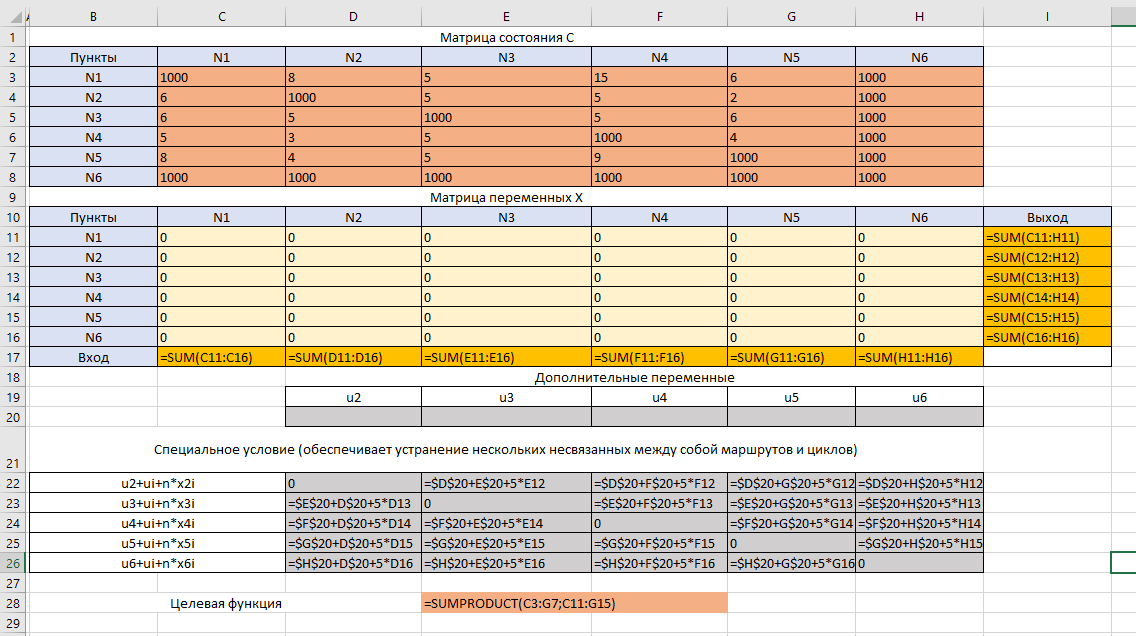
\includegraphics[width=\textwidth]{3-1.png}\\

Матрицу переменных X заполняем нулями 

В ячейку C16 запишем формулу: =СУММ(C11:C15). Автозаполнением скопируем эту формулу в ячейки диапазона D16:G16. 

В ячейку H11 запишем формулу: =СУММ(C11:G11). Автозаполнением скопируем эту формулу в ячейки диапазона H12:15. 

В ячейку F28 вводим формулу целевой функции: =СУММПРОИЗВ(C3:G7;C11:G15). В ячейки диапазона D22:G25 вводим формулы, соответствующие ограничениям: 
\begin{itemize}
	\item В ячейку E22: =\$D\$20-E20+6*E12. Автозаполнением копируем формулу в ячейки F26,G26; 
	\item В ячейку D23: =\$E\$20-D20+6*D13. Автозаполнением копируем формулу в ячейки E23, G23; 
	\item В ячейку D24: =\$F\$20-D20+6*D14. Автозаполнением копируем формулу в ячейки E24, G24; 
	\item В ячейку D25: =\$G\$20-D20+6*D15. Автозаполнением копируем формулу в ячейки E25, G25. 
	\item Ячейки D22, E23, F24, G25 = 0.
\end{itemize}

На вкладке «Данные» выбираем пункт «Поиск решения». В появившемся окне «Параметры поиска решения» (рис.2) выполняем необходимые установки: 

В поле «Оптимизировать целевую функцию» вводим абсолютный адрес ячейки F28; Направление целевой функции устанавливаем «Минимум»; 

В поле «Изменяя ячейки переменных» вводим абсолютный адрес диапазона ячеек \\\$C\$11:\$G\$15;\$D\$20:\$G\$20;
\begin{enumerate}
\item\$C\$11:\$G\$15 = бинарное 
\item\$C\$16:\$G\$16 = 1 
\item\$D\$22:\$G\$25 <= 5 
\item\$H\$11:\$H\$15 = 1 
\end{enumerate}
Устанавливаем галочку «Сделать переменные без ограничений неотрицательными» и выбираем метод решения «Поиск решения линейных задач симплекс-методом».\\

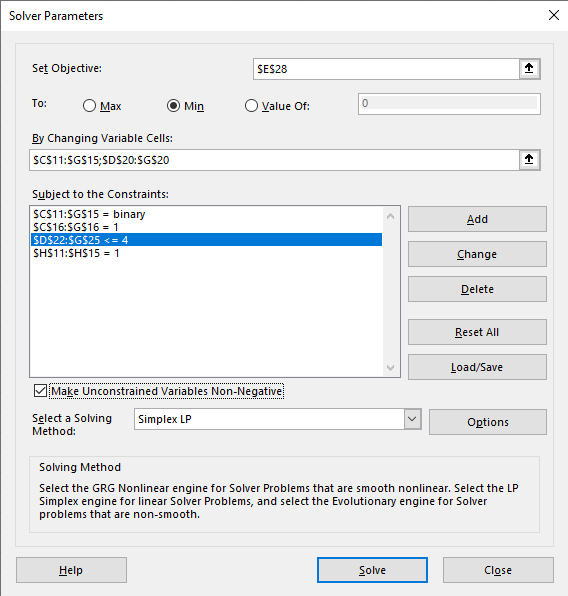
\includegraphics[width=\textwidth]{3-2.png}\\

\newpage
Нажимаем «Найти решение». Таким образом, путь:N1-N3-N4-N2-N5-N1. Минимальная длина маршрута 23.

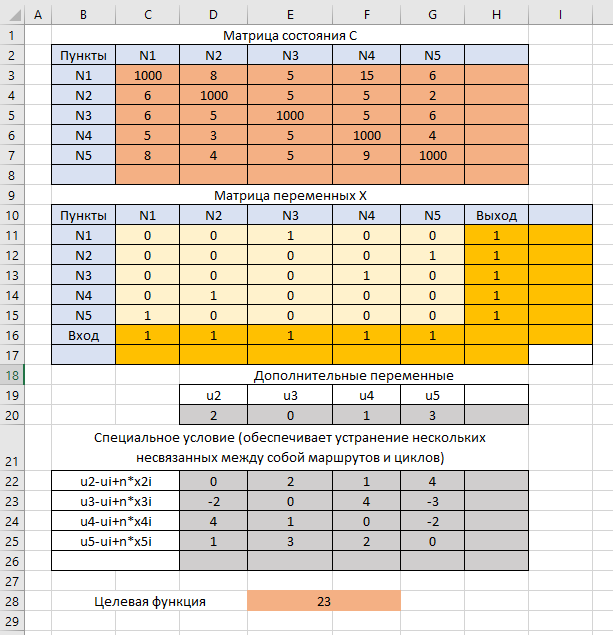
\includegraphics[width=\textwidth]{3-3.png}\\

\section{Вывод}
Задача коммивояжера может применяться для нахождения оптимального маршрута, позволяющего объехать определенные города по одному разу и вернуться в исходную точку.

\end{document}